\begin{figure*}[htb]
	\center
	\begin{subfigure}[b]{0.49\textwidth}
		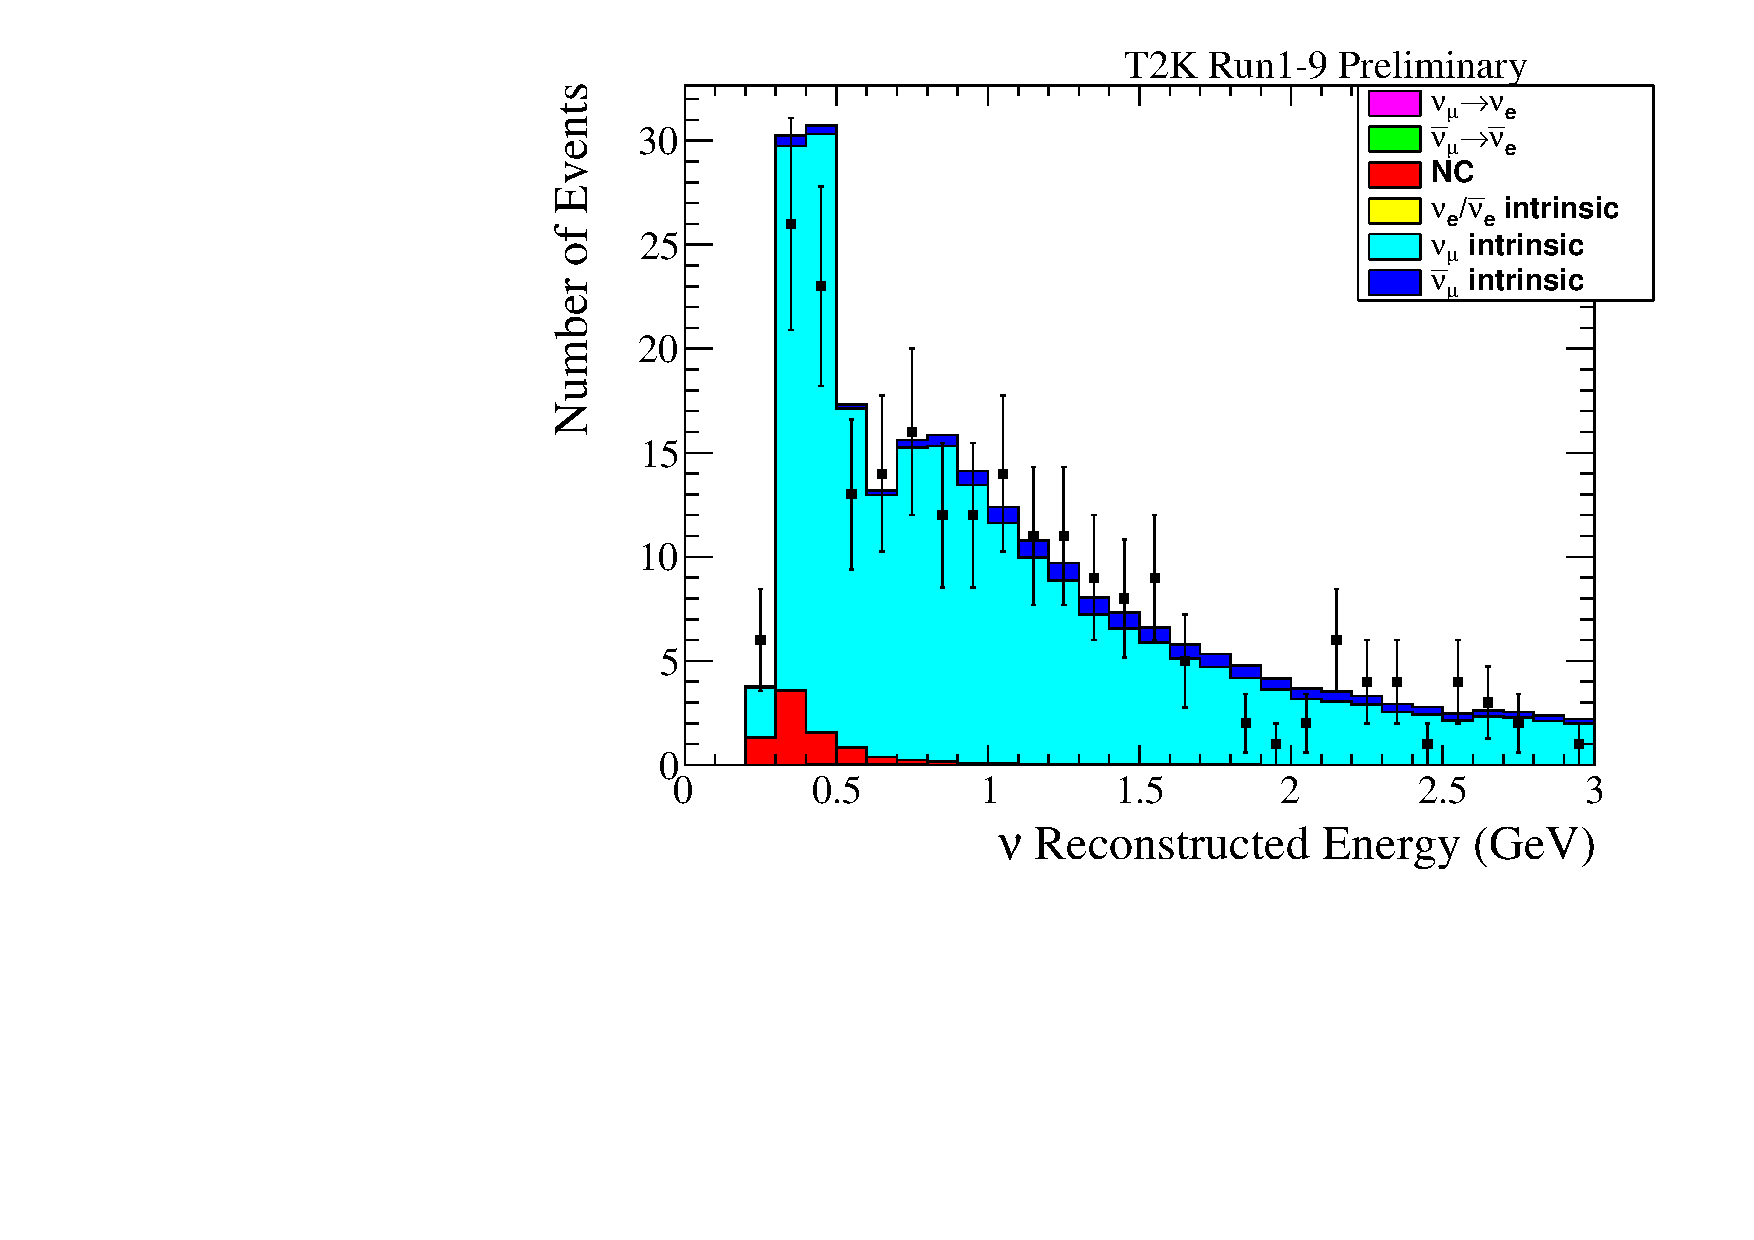
\includegraphics[width=0.9\textwidth]{spectra/Run1-9d/spectrum_AsimovA_1Rmu}
		\caption{Muon-like, neutrino mode}
	\end{subfigure}
	\begin{subfigure}[b]{0.49\textwidth}
		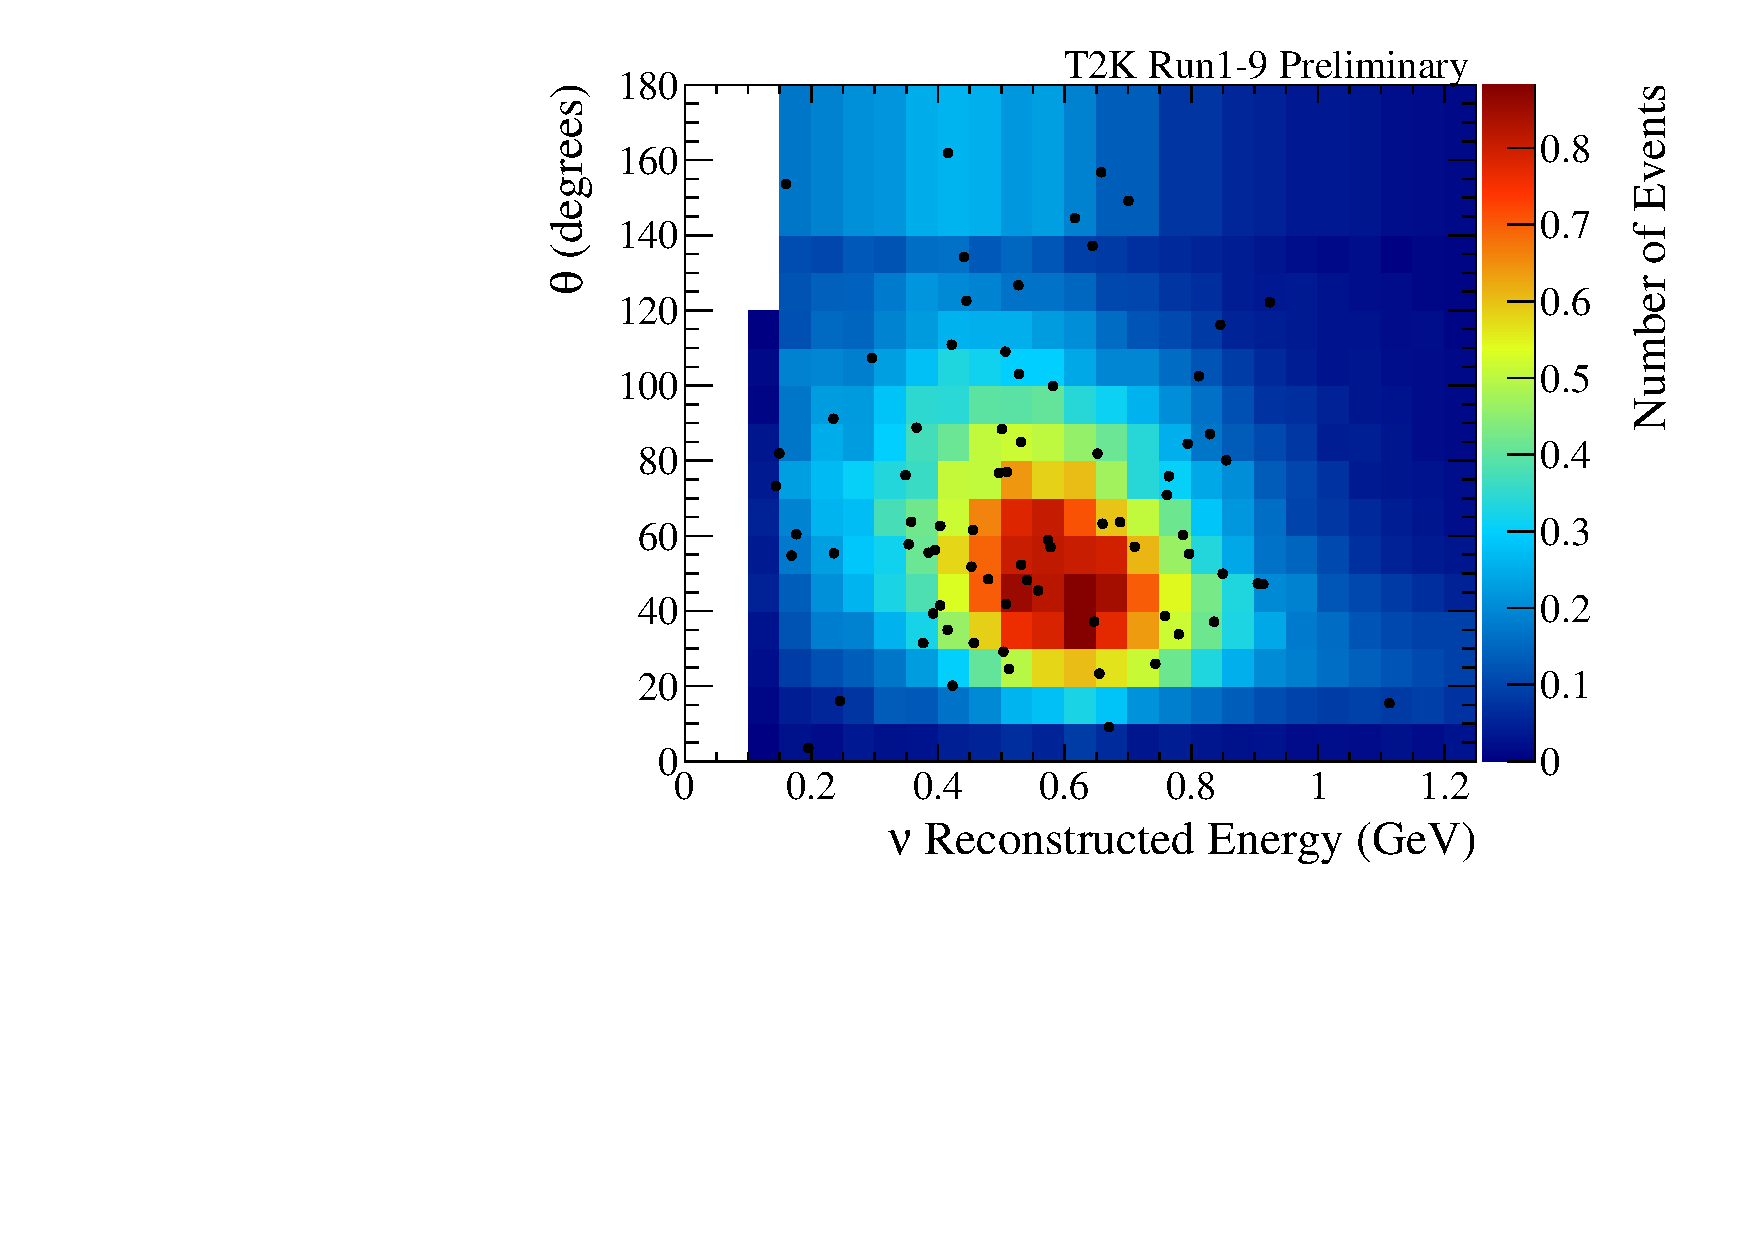
\includegraphics[width=0.9\textwidth]{spectra/Run1-9d/spectrum_AsimovA_1Re}
		\caption{Electron-like, neutrino mode}
	\end{subfigure}
	\begin{subfigure}[b]{0.49\textwidth}
		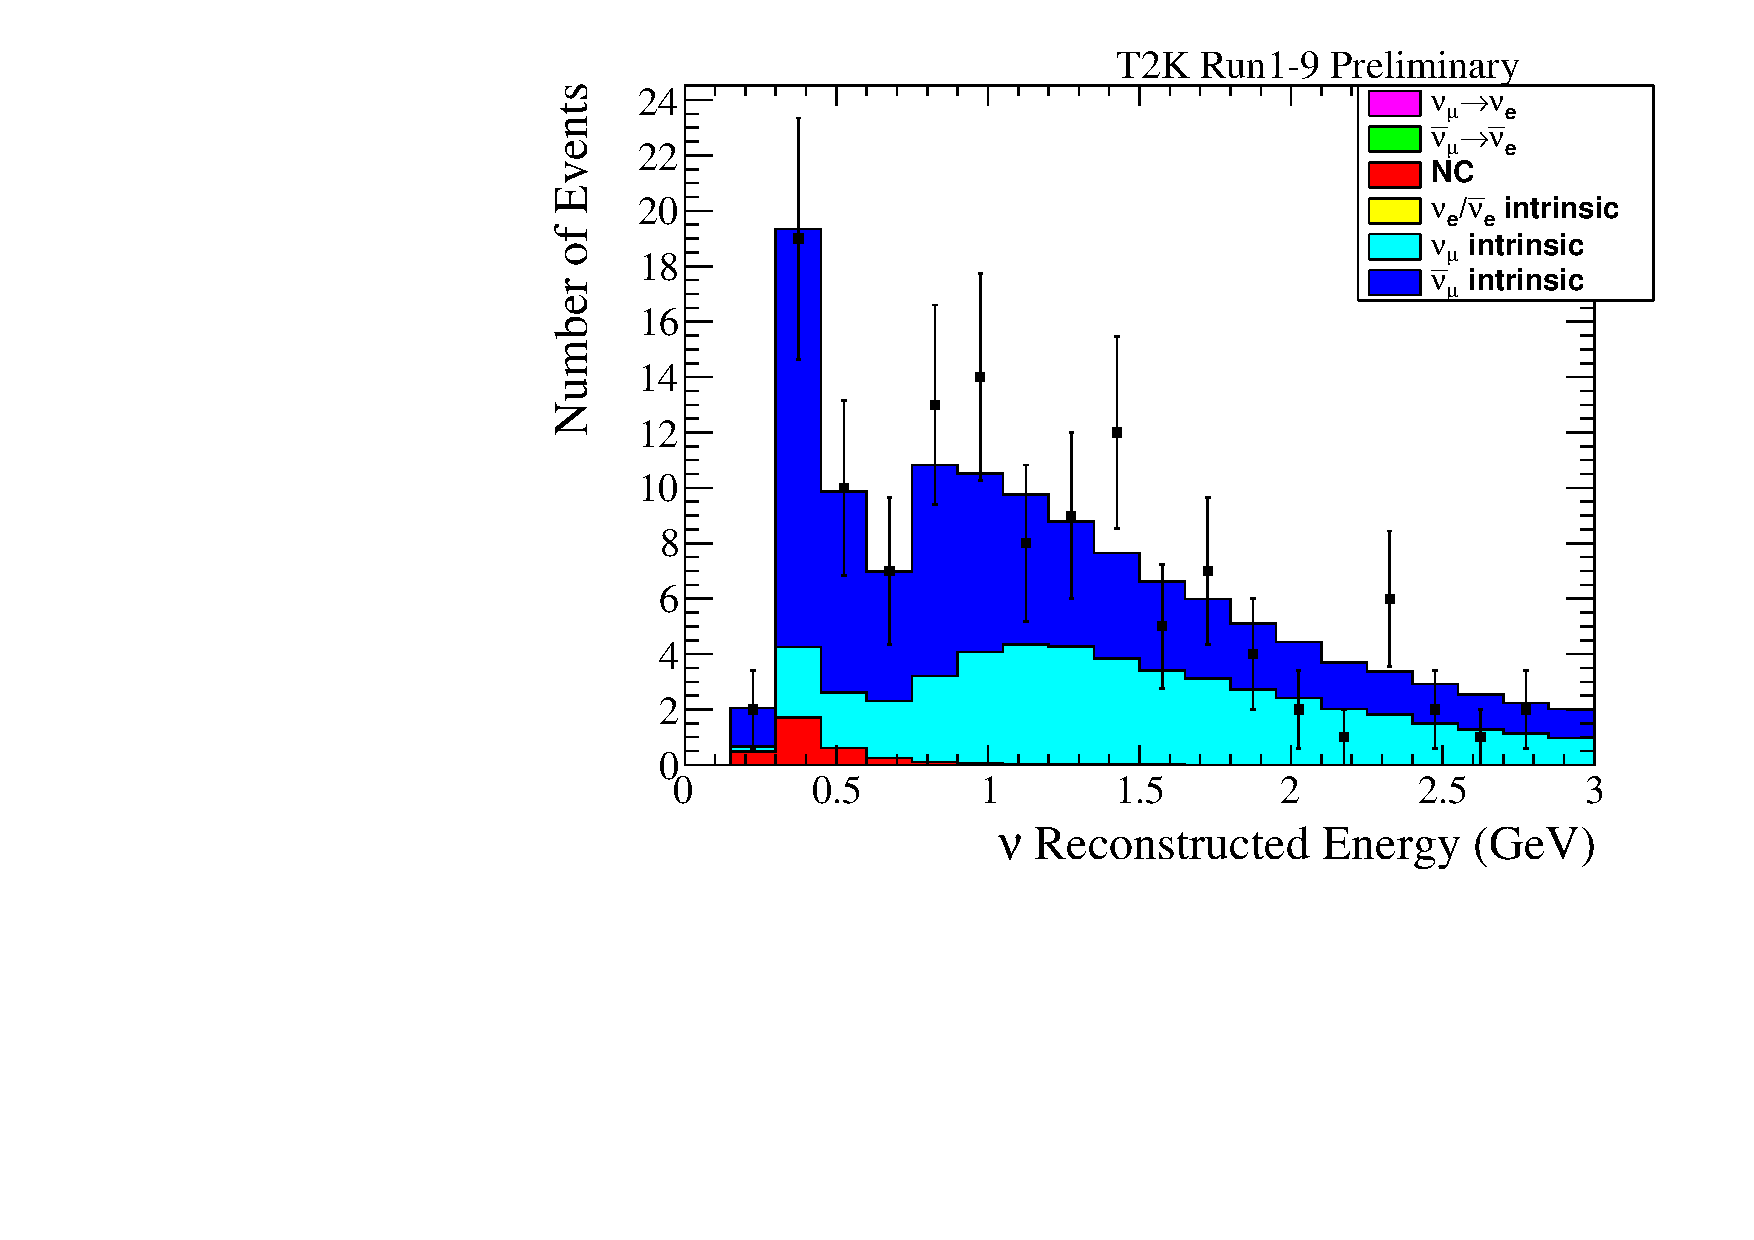
\includegraphics[width=0.9\textwidth]{spectra/Run1-9d/spectrum_AsimovA_RHC1Rmu}
		\caption{Muon-like, antineutrino mode}
	\end{subfigure}
	\begin{subfigure}[b]{0.49\textwidth}
		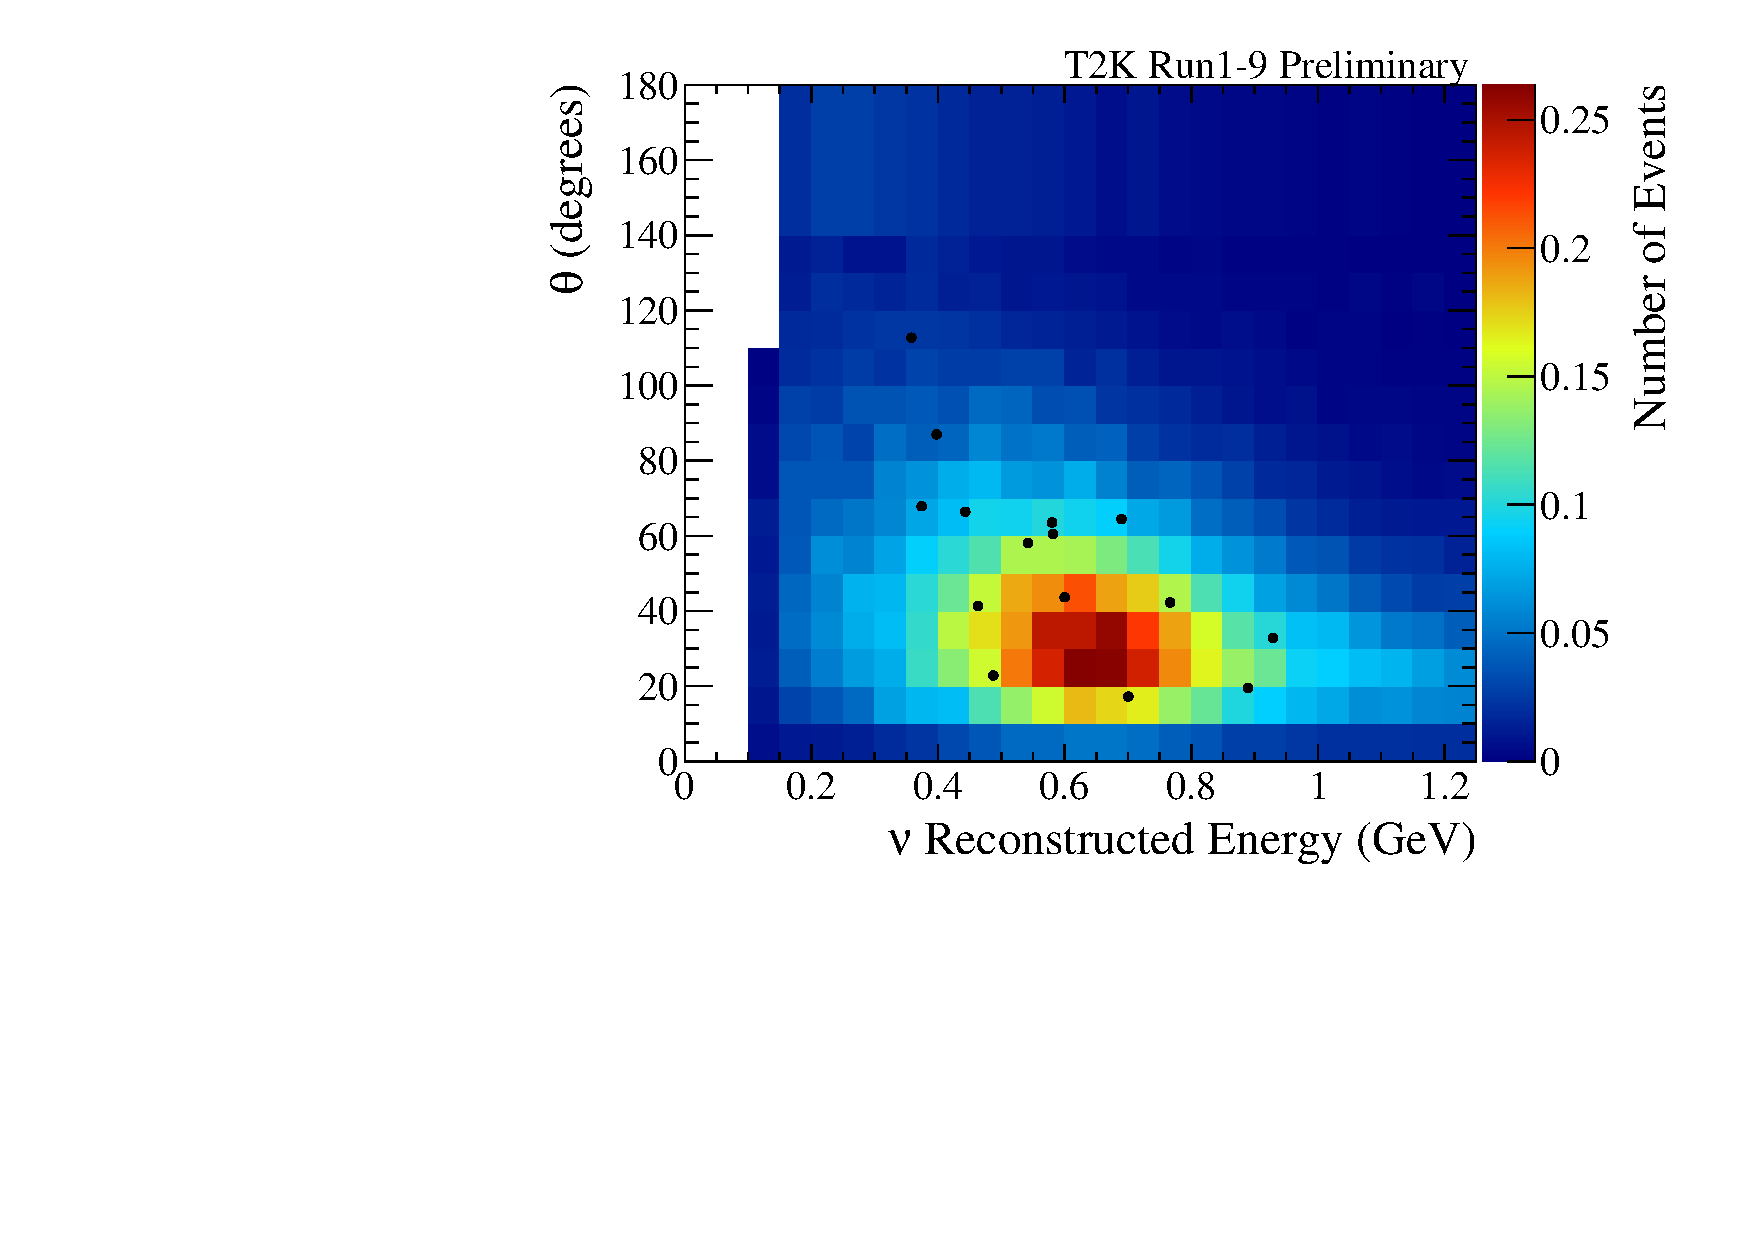
\includegraphics[width=0.9\textwidth]{spectra/Run1-9d/spectrum_AsimovA_RHC1Re}
		\caption{Electron-like antineutrino mode \label{fig:nuebar_tot_spectra_Run1-9d}}
		\label{fig:asimova_spectra_Run1-9d_RHC1Re}
	\end{subfigure}
	\begin{subfigure}[b]{0.49\textwidth}
		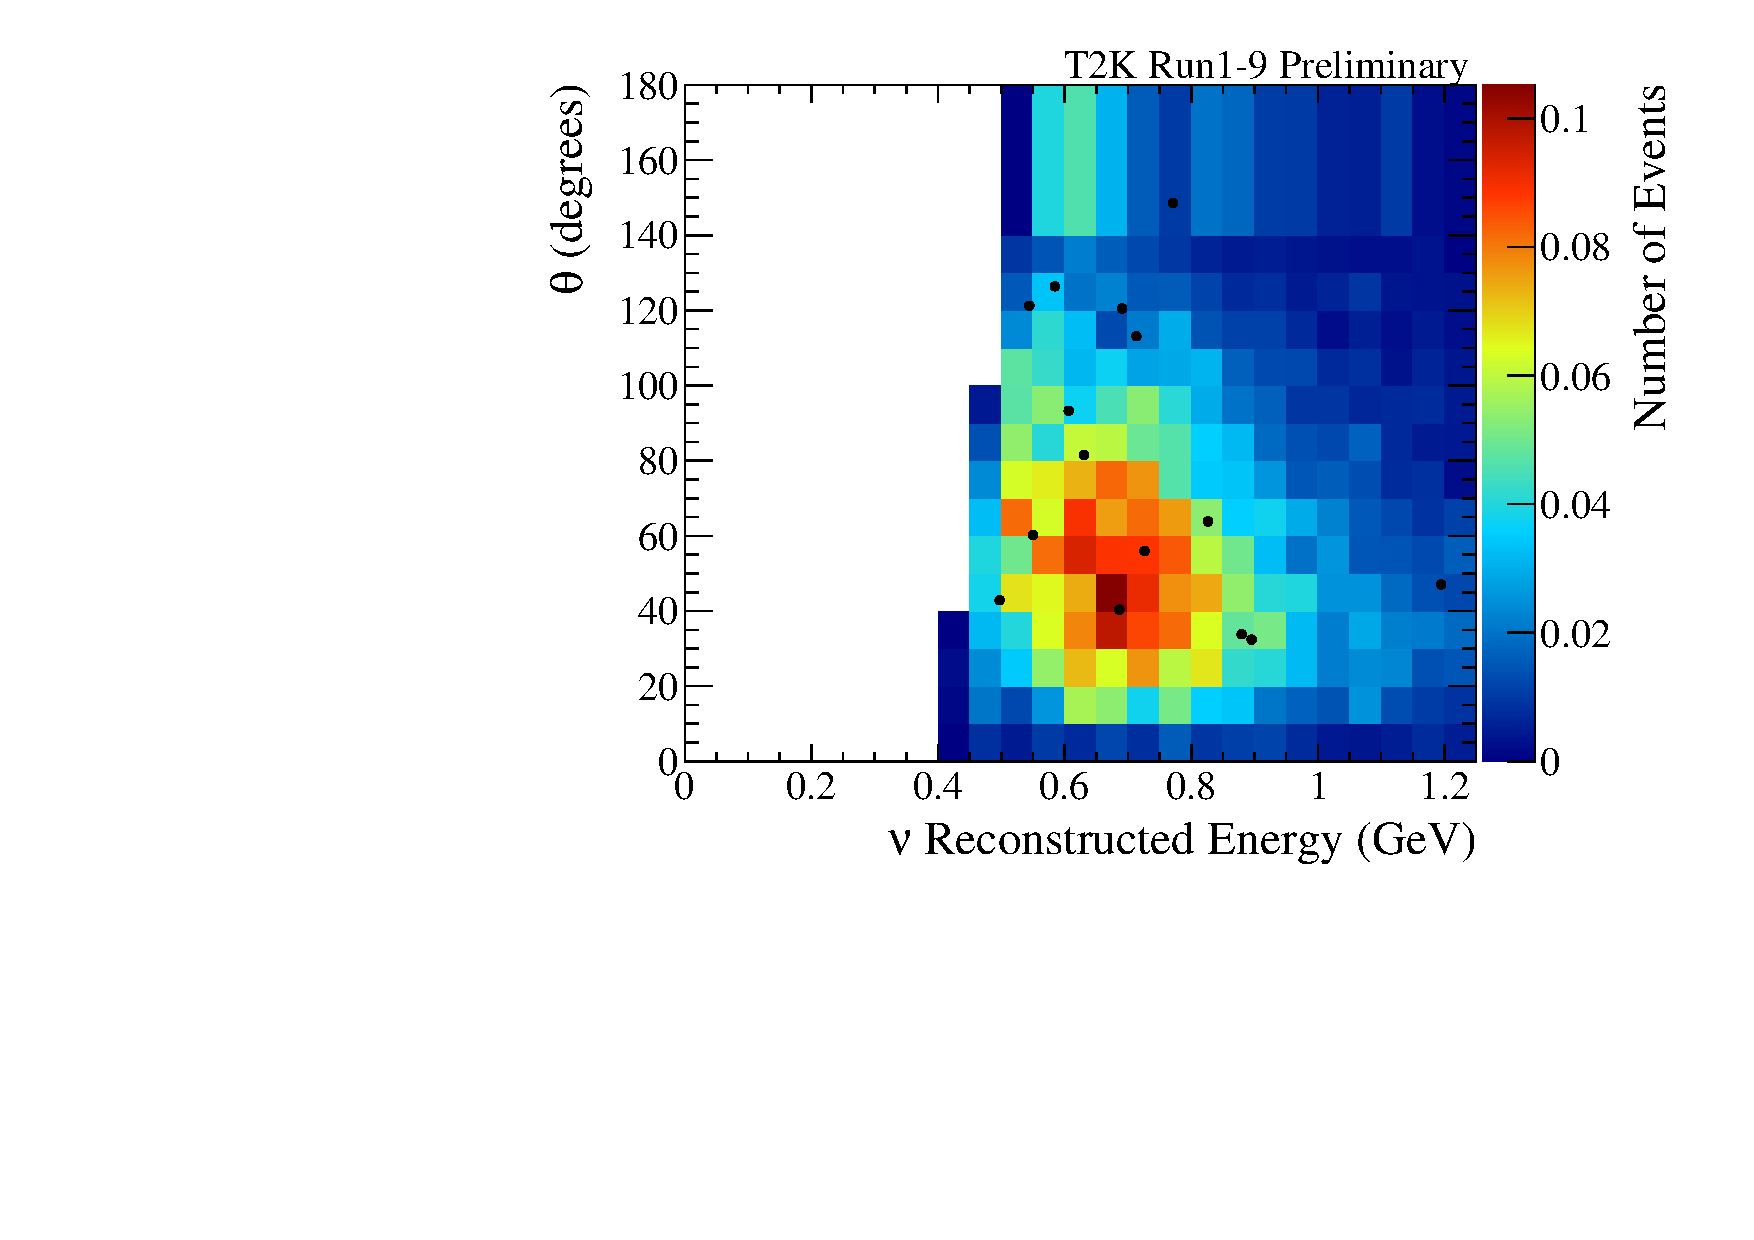
\includegraphics[width=0.9\textwidth]{spectra/Run1-9d/spectrum_AsimovA_MultiRe}
		\caption{\nueCConepi-like, neutrino mode}
	\end{subfigure}
	\caption {
		Predicted Asimov A spectra with Run 1-9 data superimposed. $\mu$-like distributions are a function of the reconstructed neutrino energy, while the $e$-like, including \nueCConepi, distributions are functions of both the reconstructed neutrino energy and the reconstructed angle between the outgoing lepton and the neutrino direction. The distributions correspond to the statistics collected in the full Run 1-9 data set. The spectra are generated with the oscillation parameters corresponding to the Asimov data set A shown in \cref{tab:osc_params_joint_asimovA}.
		%The spectra are generated with the systematic parameters described in \cref{sec:systematics} and the oscillation parameters corresponding to the Asimov data set A shown in \cref{tab:asimov_definition1}.
	}
	\label{fig:asimova_spectra_all_Run1-9d}
\end{figure*}
\clearpage